% !TEX root = main.tex

\section{Graph-based inertial-kinematic odometry}

We describe the inertial-kinematic odometry for legged robots, based on a graph model. 
Graphical methods have been extensively used for modeling estimation problems consisting of sparse networks of constraints. 
In robotics, the problems of visual odometry or simultaneous localization and mapping have reached a high degree of maturity, in great part thanks of the graphical representation. 
This is so, among other aspects, because of the power of the graphical representation to accurately model complex estimation problems. 
These often involve dynamics, proprioceptive measures, exteroceptive measures, and self-calibration. 
The graphical representation also allows for the design of powerful nonlinear estimation solvers, which can be built taking into account the needs for accuracy, robustness and CPU-performance.

\subsection{Graph-based estimation through non-linear least squares optimization}

\subsection{The inertial-kinematic odometry}

\subsubsection{Inertial pre-integration}

\subsubsection{Grahical model}

\begin{figure}[tb]
\begin{center}
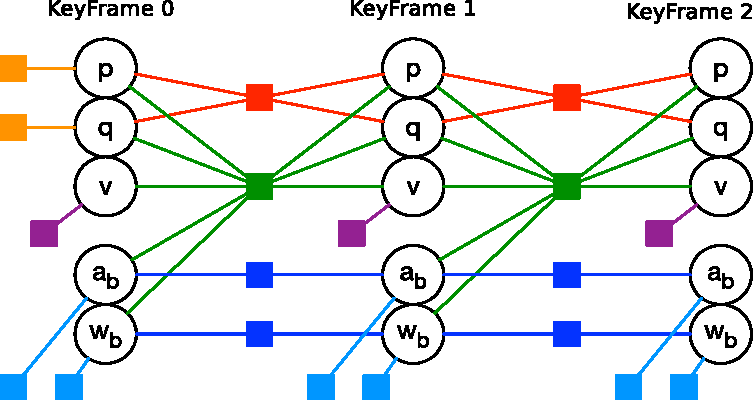
\includegraphics[scale=0.65]{figures/graph_exploded}
%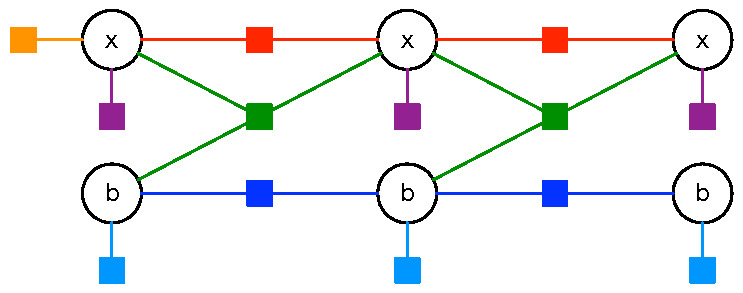
\includegraphics[scale=0.65]{figures/graph_simplified}
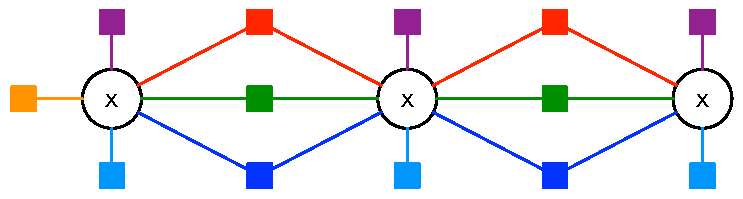
\includegraphics[scale=0.65]{figures/graph_essential}
\caption{
{\bf Top}: Detailed factor graph for the initial keyframe and two steps. \emph{Circles}: state blocks for position ($p$), orientation quaternion ($q$), velocity ($v$), accelerometer bias ($a_b$), gyrometer bias ($\omega_b$). \emph{Orange}: initial pose factor. \emph{Red}: leg kinematic factor. \emph{Green}: IMU's delta pre-integration factor. \emph{Blue}: bias drift factor. \emph{Cyan}: bias absolute factor. Purple: zero-velocity factor. 
%{\bf Mid}: Simplified factor graph where aggregate state blocks $x=(p,q,v)$ and biases $b=(a_b,\omega_b)$ are used. 
{\bf Bottom}: Equivalent factor graph with one aggregate state block $x=(p,q,v,a_b,\omega_b)$ for each key-frame. All factors are affecting exactly the same variables as in the Top graph.
}
\label{default}
\end{center}
\end{figure}

%\begin{figure}[htbp]
%\begin{center}
%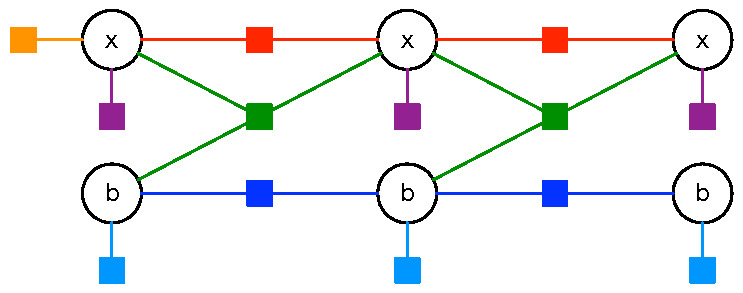
\includegraphics[scale=0.65]{figures/graph_simplified}
%\caption{default}
%\label{default}
%\end{center}
%\end{figure}

